\subsection{Details und Implementation}

\begin{center}
\emph{{\small Sascha Bachmann}}
\end{center}

\bigskip

\noindent Nachdem im vorigen Abschnitt der Marching Cubes Algorithmus allgemein beschrieben wurde, wird im Folgenden auf wichtige Details und auf die konkrete Implementation genauer eingegangen. Der Algorithmus wurde auf Grundlage der Quellen \cite{MC} und \cite{MCADD} implementiert, auf die an geeigneten Stellen noch präziser verwiesen wird.
\medskip

\subsubsection*{Übersicht} Bevor einige Aspekte der Implementation detailliert beschrieben werden, gibt zunächst die folgende Grafik einen Überblick über den Ablauf der Oberflächen-Berechnung.

\noindent
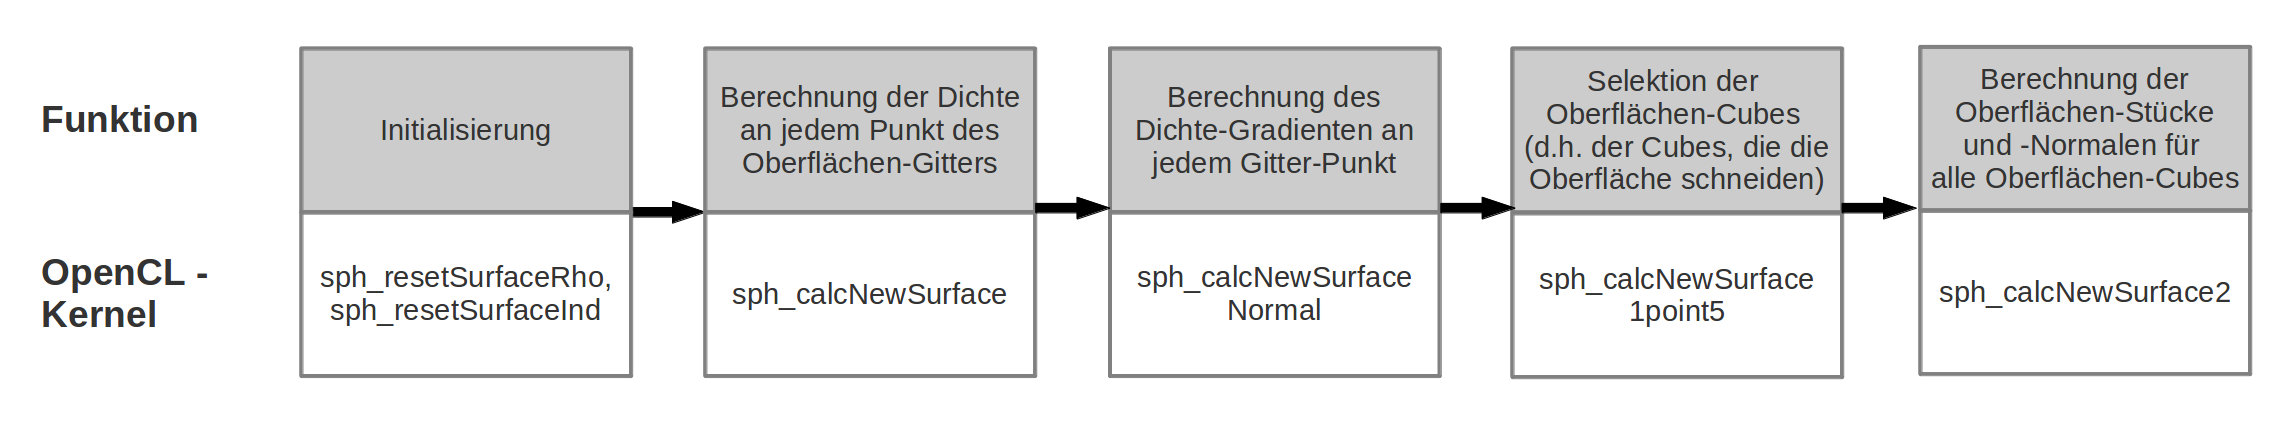
\includegraphics[scale=0.27]{images/MC-Ablauf}
\medskip

\subsubsection*{Berechnung der Gitter-Punkt-Dichten}
Nach der Initialisierung einiger OpenCL-Buffer wird im Kernel {\tt sph\_calcNewSurface} die Dichte an jedem Punkt des Oberflächen-Gitters approximiert. Hierzu wird für jeden Gitter-Punkt $x$ die Dichte $\rho_x$ mittels Gleichung \ref{density} berechnet, also
\begin{align*}
\rho_x = \sum_{i=1}^n m w(x - r_i, h).
\end{align*}
Der naive Ansatz wäre nun, dass je Work-Item sequentiell die obige Summe für einen Gitter-Punkt $x$ berechnet wird. Dies führt allerdings dazu, dass viele Work-Items nichts zu tun haben -- nämlich immer dann, wenn sich der zugehörige Gitter-Punkt außerhalb der Flüssigkeit befindet. Um die Parallelität zu erhöhen hat es sich daher als sinnvoll herausgestellt, für jeden Flüssigkeits-Partikel $i$ ein Work-Item zu starten. In einem OpenCL-Buffer sollen nun für jeden Gitter-Punkt $x$ die Dichten $\rho_x$ abgelegt werden. Hierzu bildet jedes Work-Item die Summanden $m w(x-r_i, h)$ der obigen Dichte-Summe für alle benachbarten Gitter-Punkte $x$ und addiert jeden dieser Summanden mittels der {\tt atomic\_add}-Funktion an die zu $x$ gehörende Stelle des Dichte-Buffers. Es sei noch angemerkt, dass hierbei die Summanden zunächst geeignet skaliert werden, da die {\tt atomic\_add}-Funktion nur Integer-Werte addieren kann.

\subsubsection*{Berechnung der Dichte-Gradienten}
Die Berechnung der Dichte-Gradienten im OpenCL-Kernel {\tt sph\_calcNewSurfaceNormal} erfolgt nach der in \cite[S. 165]{MC} beschriebenen Methode. Jedes Work-Item ist hierbei für die Berechnung des Gradienten an einem der Gitter-Punkte zuständig.
\medskip

\subsubsection*{Selektion der Oberflächen-Cubes}
Nachdem Dichte und Gradienten an den Gitter-Punkten berechnet wurden, kann prinzipiell die Berechnung der Oberflächen-Stücke für jeden Cube des Gitters durchgeführt werden. Hierzu soll sinnvollerweise in einem OpenCL-Kernel für jeden Cube ein Work-Item gestartet werden. Allerdings ist für diejenigen Cubes, die entweder ganz innerhalb oder ganz außerhalb der Flüssigkeit liegen, keine Oberfläche zu berechnen. Bevor daher mit der eigentlichen Oberflächen-Berechnung begonnen wird, werden die Cubes, die tatsächlich von der Oberfläche geschnitten werden, zunächst selektiert. Hierzu wird im Kernel {\tt sph\_calcNewSurface1point5} für jeden Cube des Gittes ein Work-Item gestartet. Jedes Work-Item überprüft nun, ob entweder alle Ecken des Cubes in der Flüssigkeit liegen (d.h. die Dichte an allen Ecken ist größer als ein vorgegebener Schwellenwert) oder ob alle Ecken außerhalb der Flüssigkeit liegen. Tritt einer der beiden Fälle ein, so wird in einem OpenCL-Buffer an der zum betrachteten Cube gehörenden Stelle eine $1$ eingetragen, anderenfalls eine $0$. Anschließend wird dieser Buffer Host-seitig verarbeitet und die Indizes der $0$-Einträge an den Kernel {\tt sph\_calcNewSurface2} übergeben, der für die eigentliche Oberflächen-Berechnung zuständig ist.
\medskip

\subsubsection*{Berechnung der Oberflächen-Stücke und -Normalen}





